\documentclass{article}
\usepackage[utf8]{inputenc}

\title{Category Theory for All}
\author{Valeria de Paiva \and Harley Eades III}
\date{December 2015}

\usepackage{natbib}
\usepackage{graphicx}

\begin{document}

\maketitle

\section{Introduction}
There is a theory which states that if ever anyone discovers exactly what the Universe is for and why it is here, it will instantly disappear and be replaced by something even more bizarre and inexplicable.
%There is another theory which states that this has already happened.

Category theorists believe that all can be explained with a few well chosen mathematical concepts, starting with category, functor, natural transformatins. In this or the opposite order. The aim of this work is to create a basic Lego-like library  of category theory concepts, that is latexed inan easy way to incentivate creative reuse. 

Thus we intend to have a `wordnet' of categorical concepts organized via GitHub in such a way that people can extend it to their own purposes. This definition-net of categorical concepts is meant to help us with our own work, when we put the basic bricks together in different structures.

The sources for this work are the projects on a Encyclopedia of Proof Systems, the TPTP projects, WordNet and their successors, and more distantly, the polymath projects and even Bourbaki. Of different style of contents, but similar model, another inspiration is Joshua Levy's "The command Line Guide".

One of the reasons why this might work is that any initial amount we managed to do, will already be useful for the actual mathematical work ahead. 

Right now we believe the format will be short sections, each one  with one definition, like a dictionary. We start with the definitions in \citep{depaiva1996}, which are needed for work we're doing on constructive temporal logic.

\section{Category}

\bibliographystyle{plain}
\bibliography{references}
\end{document}
\begin{figure}[h!]
\centering
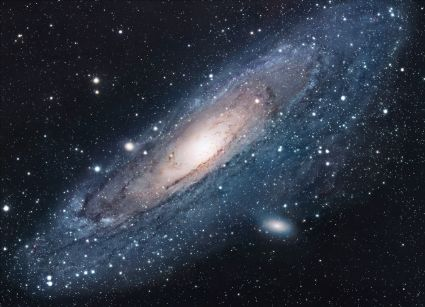
\includegraphics[scale=1.7]{universe.jpg}
\caption{The Universe}
\label{fig:univerise}
\end{figure}
``I always thought something was fundamentally wrong with the universe'' \citep{adams1995hitchhiker}
